The aim of the experiment was to gather forearm surface EMG data in
real-time, and to relate it to $(a)$ the type of grasp applied by the
subject, $(b)$ the force applied by the subject while grasping.

\subsubsection{General setup description}

The experiment consisted of freely, repeatedly grasping a SpaceControl
OFTS force/torque sensor \cite{ofts} orthogonally to its large
face. Four different ways of pressing were allowed: opposing the thumb
and index, the thumb and middle, the thumb and ring or the thumb and
all other fingers, at different speeds and with varying force. Four
force sensing resistors (FSRs) were applied on the subject's hand
fingertips (thumb, index, middle and ring), in order to be able to
detect which grasp type was used at each instant of time. At the same
time, $10$ forearm surface EMG electrodes were applied to the
subject's forearm, held in place by elastic bands, in order to gather
information about the muscle activation. Figure \ref{fig:setup} shows
some parts of the setup.

\begin{figure} \centering
  \begin{tabular}{cc}
    %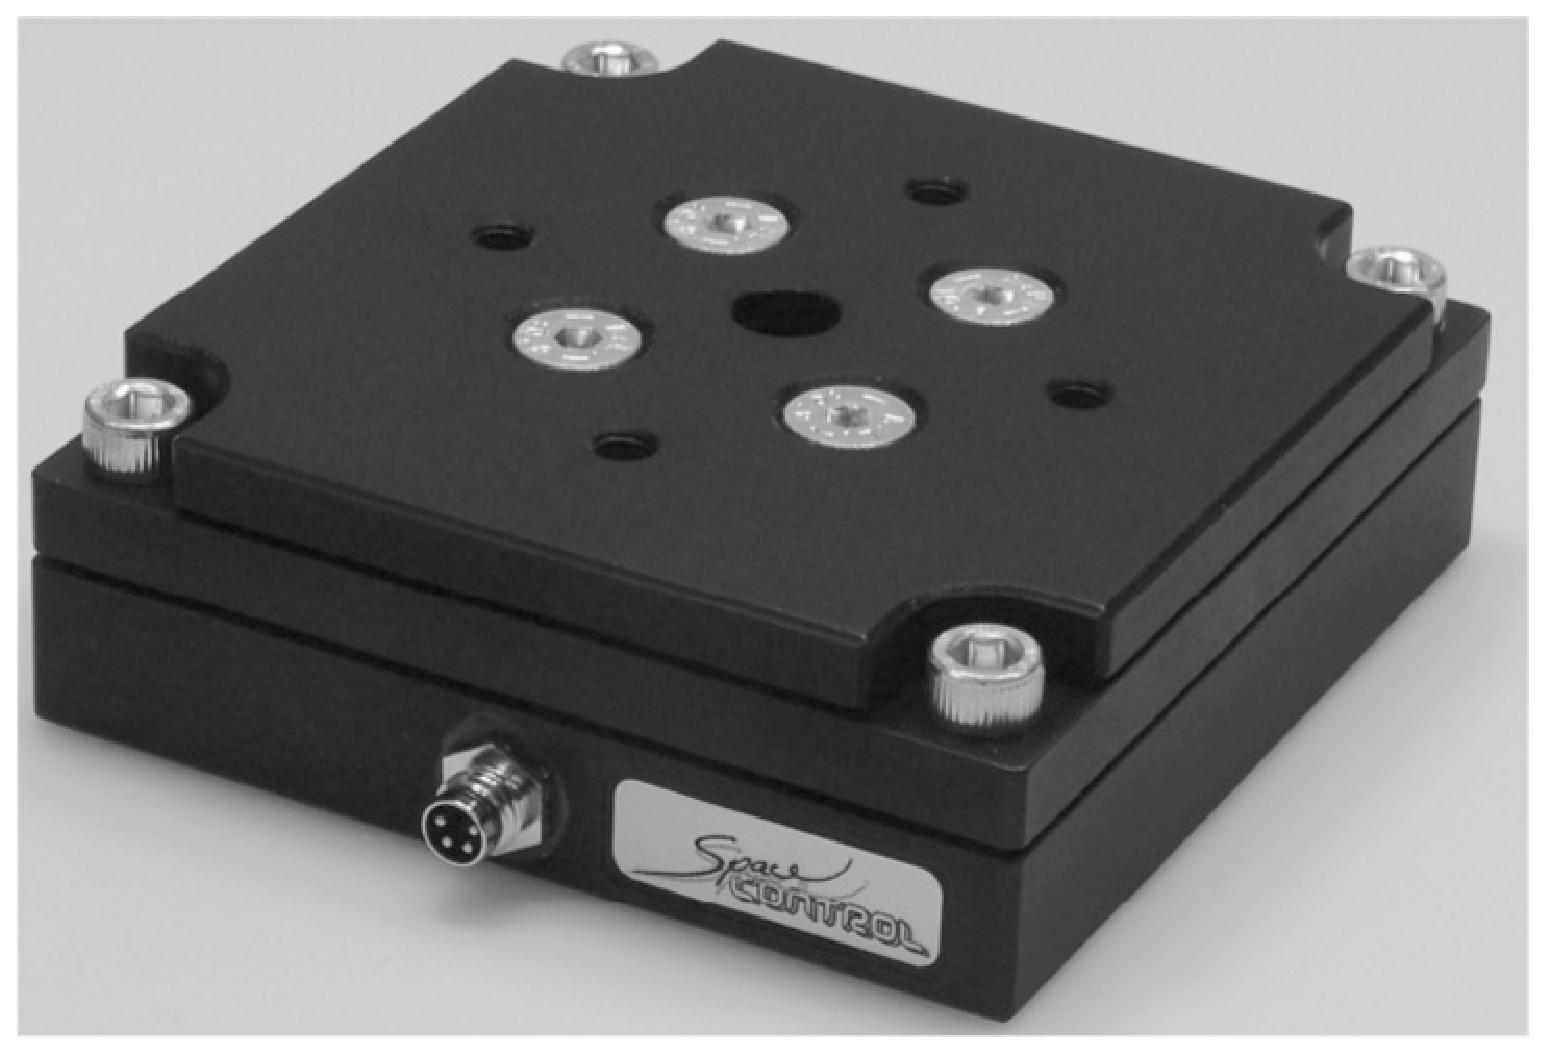
\includegraphics[height=0.12\textheight]{figs/OFTS} &
    
\includegraphics[height=0.12\textheight]{figs/ottobock} &
    
\includegraphics[height=0.12\textheight]{figs/setup} \\
    $(a)$ & $(b)$\\
  \end{tabular}
  \caption{The experimental setup. $(a)$ An Otto Bock 13E200=50
    surface EMG electrode. $(b)$
    The arm of the subject with the EMG electrodes fitted and held in
    place by elastic bands.}
  \label{fig:setup}
\end{figure}

Numerical data from the EMG electrodes and FSRs were gathered at a
sampling rate of $256$Hz using a National Instruments DAQ PCI-6023E
analogic/digital conversion card \cite{nidaq}, mounted on a fast PC
equipped with Windows XP. Data coming from the OFTS sensors was
gathered via the serial port at about $80$KHz. The data were
subsequently synchronised.

\subsubsection{EMG signal and electrode placement}

The $10$ EMG electrodes were applied to the subject's right forearm,
held in place by elastic bands. The electrodes were
double-differential Otto Bock 13E200=50 models \cite{ottobock}, used
at an amplification factor of about $14,000$. Six of the electrodes
were placed in pairs along the lower face of the forearm, whereas four
of them were applied in pairs on the upper face. Placement was done
following the description in \cite{smagt}, which proved to be optimal
for Support Vector Machine classification of hand postures.

As far as the EMG signal is concerned, it must be remarked that it is
subject to remarkable changes depending on, at least, four orders of
factors: (1)~the subject, (2)~the arm posture, (3)~electrode
placement, and (4)~muscle fatigue. As far as the first problem is
concerned, since in a real setting one person only is expected to
train and wear the prosthesis, we have not investigated multi-subject
feasibility of the approach, concentrating on one subject only, male,
aged $35$ and fully able-bodied. In subsequent work, independent
multi-subject analysis will have to be carried on.

In order to overcome the second problem, we instructed the subject to
keep the arm still and relaxed on a table in a comfortable position,
with the palm orthogonal to the plane of the table. Again, a deeper
investigation is required in a real setting, since the prosthesis is
supposed to be worn all day long in all possible tasks of everyday
life.

%
%Lastly, as far as muscle fatigue and electrode displacement are
%concerned: in general, electrodes \emph{cannot} be expected to exactly
%lie in the very same position every time the prosthesis is used;
%moreover, in a preliminary round of experiments, muscle fatigue was
%clearly perceived by the subject during the experiment. In this
%framework, the only possibility to overcome these problems is to
%explicitly take them into account, gathering enough data to be able to
%train the machine under different conditions of electrode displacement
%and muscular fatigue.

We then organised the experiment as follows: the subject was
instructed to continually grasp the sensor over a period of time of
$3$ to $4$ minutes; then he was allowed to rest for about two
minutes. This was called a \emph{session}. It was expected that muscle
fatigue would appear already during one session.

Three sessions were gathered without taking the elastic bands off the
subject's forearm, in order \emph{not} to have electrode displacement
within such a set of sessions, that we called a \emph{group}. After
each group, the electrodes and bands were removed and the subject was
allowed for a much longer period of rest, ranging from half an hour to
one hour. During resting in-between groups, the subject could get back
to his normal muscular activity.

Five groups were then gathered during one day; and this procedure was
entirely repeated during another day. This procedure would allow us to
examine a relevant amount of data, gathered along a relatively long
period of time and under different conditions of muscle fatigue
(within one session) and electrode displacement (between groups).

%As an example, Figure \ref{fig:drift} shows the typical electrode
%output during three different sessions: $1$ and $2$, belonging to
%the same group, and $7$ (moving average over about $10$ seconds).
%One can notice strong low-frequency components, essentially drifts
%due to muscle fatigue. As a matter of fact, a spectral analysis of
%the signal shows that most of the relevant information is
%contained in the range $0$ to 20--30Hz, therefore sampling at
%$256$Hz proved later on to be a large overshoot.
%
%\begin{figure*}[!ht] \centering
%  \begin{tabular}{ccc}
%    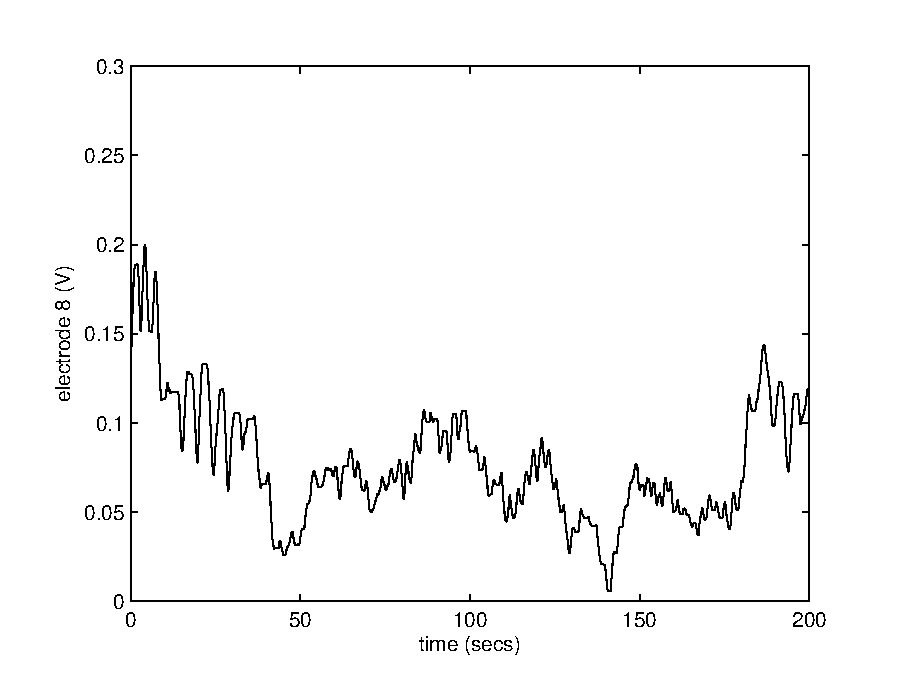
\includegraphics[width=0.32\textwidth]{figs/el8_movingAvg_s1} &
%    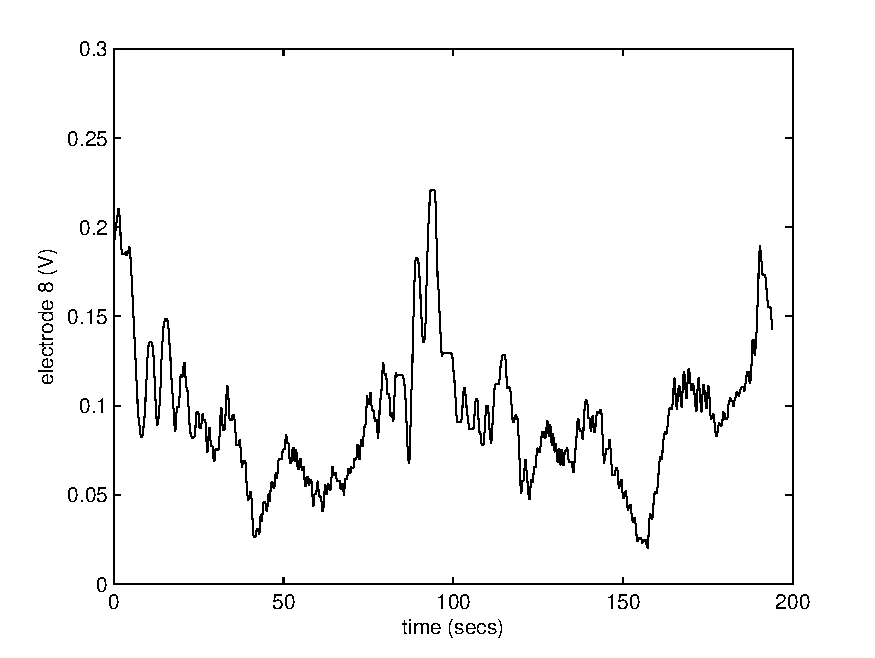
\includegraphics[width=0.32\textwidth]{figs/el8_movingAvg_s2} &
%    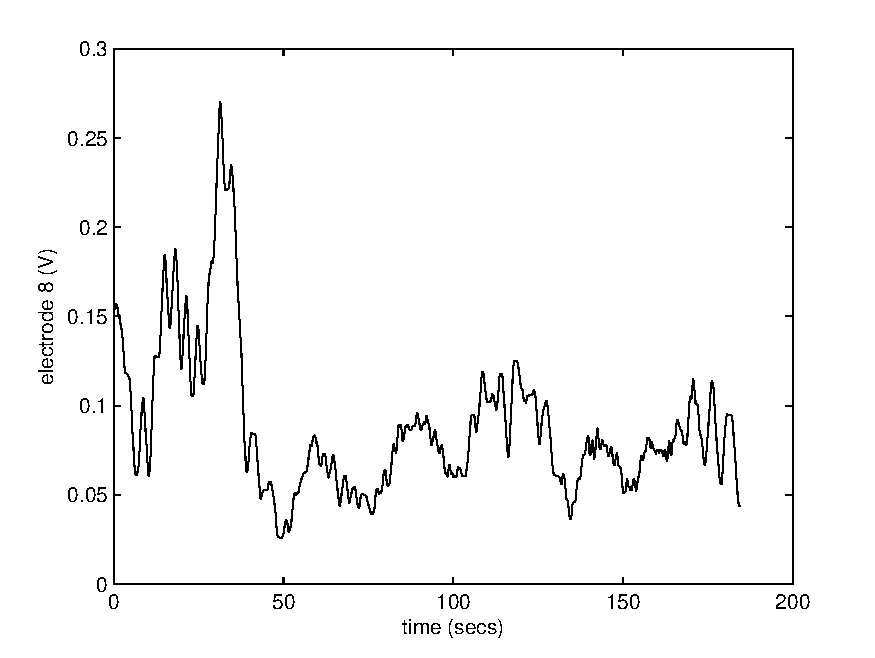
\includegraphics[width=0.32\textwidth]{figs/el8_movingAvg_s7} \\
%    Session $1$ & Session $2$ & Session $7$ \\
%  \end{tabular}
%  \caption{Typical behaviour of an electrode signal over different
%  sessions (moving average over about $10$ seconds). Drifting can be
%  clearly seen in the signal, due to muscle fatigue.}
%  \label{fig:drift}
%\end{figure*}

\subsubsection{Force applied during the grasp}

The output of the linear OFTS force/torque sensor lies between 0N
and 100N, with a resolution of $0.02$N.

\subsubsection{Type of grasp}

The voltage values output by the $4$ FSRs applied onto the subject's
fingertips were monitored in order to understand which kind of grasp
the subject was applying to the sensor. A threshold was experimentally
decided, above which the finger would be defined \emph{in contact}
with the sensor. Using this technique, for each instant in time one of
five possible categories was established: $0$, no action; $1$, grasp
by opposing the thumb and index finger; $2$, opposing thumb and
middle; $3$ thumb and ring; and lastly $4$, grasp by opposing the
thumb and all other fingers.
%
%It must be remarked here that the EMG signal would be altered
%immediately at the onset of finger movement, which our setup was
%unable to detect. This would result in potential wrong EMG values for
%category $0$. Moreover, the FSRs have been experimentally determined
%to suffer from a remarkable hysteresis effect, that is, they will
%indicate slightly different voltage when the subject is pressing and
%when he is releasing; this is most likely due to small rubber ends
%glued on top of the sensor surfaces which would improve the grasping
%feeling of the subject. Hysteresis is also supposed to somehow degrade
%the quality of the learning. Because of these factors we would never
%expected a close-to-$100\%$ classification accuracy, nor a perfect
%reconstruction of the applied force. A better setup is currently being
%studied, which would avoid these effects.

%Figure \ref{fig:targets} shows typical values of the OFTS sensor and
%the related categories. One can clearly see that the applied force is
%in general higher when grasp type $4$, all fingers involved, is used,
%as expected.
%
%\begin{figure*}[!ht] \centering
%  \begin{tabular}{cc}
%    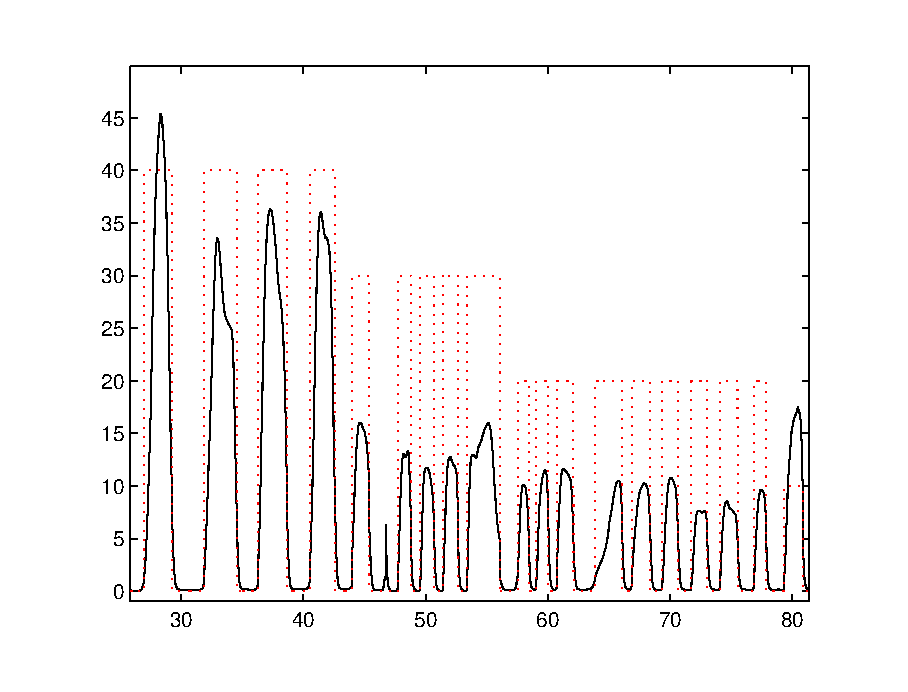
\includegraphics[width=0.4\textwidth]{figs/targets_zoom1} &
%    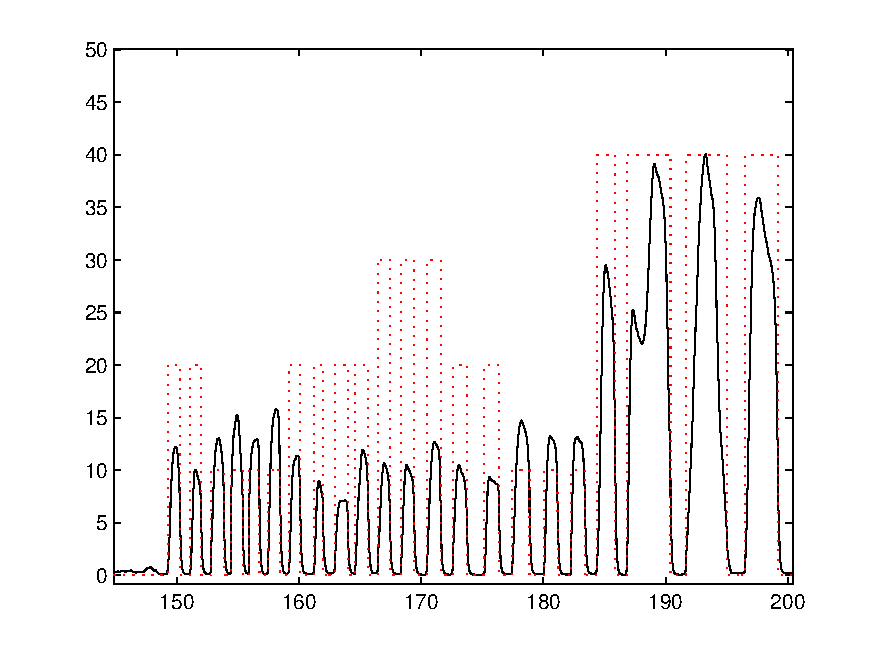
\includegraphics[width=0.4\textwidth]{figs/targets_zoom2} \\
%  \end{tabular}
%  \caption{Typical values output by the OFTS sensor (solid line), and the
%    categories evaluated from the fingertip sensors values (dotted
%    line). The Figures are zooms of the same session.}
%  \label{fig:targets}
%\end{figure*}
